% paper/v2/main.tex -- rewritten from scratch in P7 from results/P7/CLAIMS.md and results/P7/TABLES.md.
% Every number in this file must appear in results/P7/TABLES.md: run `python3 -I tools/paper_numbers_check.py`.
% Title options (working title = option 1; to be confirmed with the supervisor):
%   1. Frequency-Based Replacement for DLRM Embedding Caches: A Trace-Driven Study and a Synthesizable LFU Controller
%   2. Does LFU Help DLRM Embedding Caches? Per-Table and Shared-Cache Trace Simulation on Criteo, with an Open-PDK
%      LFU Controller
%   3. Reset-on-Eviction LFU for Shared Embedding Caches: Criteo Trace Simulation and a Gate-Level-Verified
%      Controller on NanGate45
\documentclass[conference,10pt]{IEEEtran}
\usepackage[T1]{fontenc}
\usepackage{mathptmx}
\usepackage{graphicx}
\usepackage{amsmath}
\usepackage{booktabs}
\usepackage{cite}
\usepackage{url}
\usepackage{xcolor}
\usepackage{tikz}
\usetikzlibrary{positioning,arrows.meta,fit,calc}
\usepackage[final]{microtype}
\graphicspath{{figs/}}
\DeclareUrlCommand\src{\urlstyle{tt}}

\begin{document}

\title{Frequency-Based Replacement for DLRM Embedding Caches: A Trace-Driven Study and a Synthesizable LFU
Controller\\[2pt]{\normalsize [Working title, to be confirmed]}}

\author{\IEEEauthorblockN{[Author names to be confirmed]}
\IEEEauthorblockA{[Affiliation to be confirmed]}}

\maketitle

\begin{abstract}
Embedding lookups in deep-learning recommendation models (DLRMs) touch a few rows far more often than the rest,
which makes caching them attractive, but which replacement policy to use is an open question. We compare seven
policies by trace simulation on the first 2,000,000 and the first 10,000,000 rows of the 45,840,617-row Criteo
Display Advertising Challenge training file, with either one cache per table or one cache shared by all 26 tables.
With a 256-vector cache per table, both LFU variants beat LRU (LFU with per-address counters kept after eviction:
71.8034\% vs.\ 67.3151\% hits at 2M rows, 68.3280\% vs.\ 67.0796\% at 10M). With one shared 256-entry cache, LFU
that resets an address's count on eviction beats LRU (47.6719\% vs.\ 41.4010\% at 2M, 48.1592\% vs.\ 41.2640\% at
10M), while the variant that keeps counts does not (41.0006\%, 38.4896\%). ARC and W-TinyLFU have the highest online hit
rates at the smallest capacities in both organisations, at the price of extra state. GPU timing of 26 synthetic
EmbeddingBag tables on one H100 and one H200 used CUDA events only (no hardware counters) and is launch-bound at small
batches. We also build a synthesizable LFU cache controller whose default counter mode belongs to the
reset-on-eviction family. On the NanGate45 open cell library (not TSMC; pre-layout; area as the sum of cell areas;
no power analysis) it reaches 636.1, 603.0 and 556.6\,MHz at depths 16, 64 and 256 (counter mode 0), within a synthesis-flow noise
floor of 4.92--16.23\%. Zero-delay gate-level simulation with cell models generated from the liberty file matches
the RTL in every one of 200,000 random cycles for all 12 netlists; formal equivalence is proven at depth 16 only.
\end{abstract}

\section{Introduction}
Deep-learning recommendation models combine dense features with many categorical features, each mapped to a row of
an embedding table~\cite{naumov2019dlrm}. Characterisation of production recommendation models has shown that these
models place different demands on hardware than vision or language networks~\cite{gupta2020architectural}, and a
line of systems work exploits the skew of embedding accesses: Bandana keeps embeddings in non-volatile memory with a
DRAM cache~\cite{eisenman2019bandana}, FAE keeps frequently accessed (``hot'') embeddings in GPU
memory~\cite{adnan2022fae}, ScratchPipe builds a GPU-side embedding cache that looks at future
accesses~\cite{kwon2022scratchpipe}, and RecNMP moves embedding operations near memory~\cite{ke2020recnmp}. Each of
these needs a rule for which rows to keep. Skew suggests frequency-based replacement (LFU) rather than recency (LRU),
but LFU comes in variants that behave differently, and the organisation of the cache (one per table or one for all
tables) changes the competition between tables.

This paper reports a trace-driven comparison and a hardware building block, and states the limits of each next to
the result:
\begin{itemize}
\item A comparison of LRU, two LFU variants, TinyLFU with exact counters, W-TinyLFU, ARC and Belady's offline bound
on Criteo traces, for per-table and shared caches, at two trace lengths (Sections~\ref{sec:sim}, \ref{sec:res-sim}).
\item The finding that the ranking of the two LFU variants depends on the cache organisation, and that ARC and
W-TinyLFU are the strongest online policies at small capacities (Section~\ref{sec:res-sim}).
\item GPU timing of embedding lookups without hardware counters, with the launch-bound region identified
(Section~\ref{sec:res-gpu}).
\item A synthesizable LFU controller, its timing and area on NanGate45 across design iterations with the flow noise
floor, and its verification by mutation testing, gate-level simulation and formal equivalence
(Sections~\ref{sec:rtl}, \ref{sec:res-hw}).
\end{itemize}
Every number in this paper is generated from committed result files (\src{results/P7/TABLES.md}); each table and
figure names its source.

\section{Background}
\textbf{LRU} evicts the least recently used entry. \textbf{LFU} evicts the entry with the fewest accesses; variants
differ in whether an address's count survives its eviction. We call the variant that discards the count on eviction
and restarts it at one on re-insertion \emph{LFU, reset on eviction}, and the variant that keeps a per-address count
in an unbounded table \emph{LFU, persistent counters}; the latter is an idealised model of history-keeping LFU.
\textbf{TinyLFU} adds an admission filter that compares the frequency of a new item with that of the eviction
candidate; \textbf{W-TinyLFU} places a small LRU window in front of the main cache~\cite{einziger2017tinylfu} and
estimates frequencies with a Count-Min sketch~\cite{cormode2005countmin}. \textbf{ARC} balances a recency list and a
frequency list and keeps ghost lists of recently evicted keys to adapt the balance~\cite{megiddo2003arc}.
\textbf{Belady's} MIN policy evicts the entry used furthest in the future; it needs the whole trace and serves as an
upper bound~\cite{belady1966study}.

\section{Trace Simulation Setup}\label{sec:sim}
\textbf{Data.} We use the Criteo Display Advertising Challenge training file (Kaggle, 2014)~\cite{criteo2014dac},
45,840,617 rows with 26 categorical columns. Each column is one embedding table and each distinct hashed value one
vector. We replay the first 2,000,000 and the first 10,000,000 rows, i.e.\ a prefix of the file; nothing is claimed
for the full file. Empty fields produce no access. Rank-frequency fits of a Zipf exponent per table give
$\alpha$ from 1.0733 to 4.9724 at 2M rows and 1.0759 to 5.6033 at 10M rows (24 of 26 tables; two tables have only
three distinct values).

\textbf{Cache organisations.} \emph{Per-table}: each table has its own cache of $C$ vectors (26 caches;
$C$ from 64 to 100,000). \emph{Shared}: one cache of $C$ entries holds vectors of all tables (key = table and
value; $C$ = 256, 1,000, 10,000 and 100,000), and the accesses of one row are issued in table order 0 to 25. The
shared ordering is a modelling choice. Capacities are in vectors, not bytes.

\textbf{Policies.} The seven policies of the previous section. TinyLFU is run with exact counters and a 1\% window;
W-TinyLFU with a Count-Min sketch and a 1\% window. The LFU variants evict the smallest count and break ties in
favour of the entry that entered the cache earliest; their counts saturate at 255. The simulators are covered by
unit tests and by mutation tests that check the tests fail on deliberately broken policies.

\section{LFU Controller}\label{sec:rtl}
\begin{figure}[t]
\centering
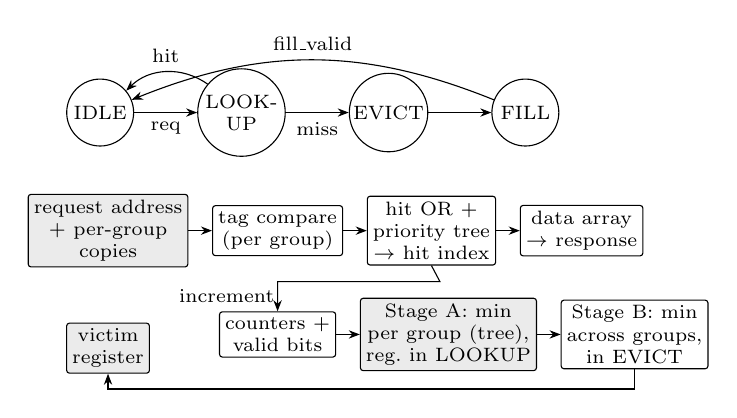
\begin{tikzpicture}[
  font=\scriptsize, >={Stealth[length=4pt]},
  blk/.style={draw, rounded corners=1pt, align=center, minimum height=5.5mm, inner sep=2pt, fill=white},
  st/.style={draw, circle, inner sep=1pt, minimum size=8.5mm, align=center},
  reg/.style={blk, fill=black!8}]
  % FSM
  \node[st] (idle) {IDLE};
  \node[st, right=8mm of idle] (look) {LOOK-\\UP};
  \node[st, right=8mm of look] (evict) {EVICT};
  \node[st, right=8mm of evict] (fill) {FILL};
  \draw[->] (idle) -- node[below]{req} (look);
  \draw[->] (look) -- node[below]{miss} (evict);
  \draw[->] (evict) -- (fill);
  \draw[->] (look) to[bend right=40] node[above]{hit} (idle);
  \draw[->] (fill) to[bend right=22] node[above]{fill\_valid} (idle);
  % datapath
  \node[reg, below=6mm of idle, xshift=1mm] (addr) {request address\\+ per-group\\copies};
  \node[blk, right=3mm of addr] (cmp) {tag compare\\(per group)};
  \node[blk, right=3mm of cmp] (hit) {hit OR +\\priority tree\\$\rightarrow$ hit index};
  \node[blk, right=3mm of hit] (data) {data array\\$\rightarrow$ response};
  \node[blk, below=7mm of cmp] (cnt) {counters +\\valid bits};
  \node[reg, right=3mm of cnt] (sa) {Stage A: min\\per group (tree),\\reg.\ in LOOKUP};
  \node[blk, right=3mm of sa] (sb) {Stage B: min\\across groups,\\in EVICT};
  \node[reg, below=7mm of addr] (vic) {victim\\register};
  \draw[->] (addr) -- (cmp);
  \draw[->] (cmp) -- (hit);
  \draw[->] (hit) -- (data);
  \draw[->] (cnt) -- (sa);
  \draw[->] (sa) -- (sb);
  \draw[->] (sb.south) -- ++(0,-2.5mm) -| (vic.south);
  \coordinate (mid) at ($(hit.south)!0.5!(sa.north)$);
  \draw[->] (hit.south) -- (mid) -| node[pos=0.75, left, inner sep=1pt]{increment} (cnt.north);
\end{tikzpicture}
\caption[]{The LFU controller (\src{rtl/v2/lfu_cache_controller.v}, tag \src{rtl-v2-final}): FSM (top) and datapath
(bottom; shaded blocks are registers). A hit returns to IDLE; a miss selects the victim (Stage A registered in
LOOKUP, Stage B in EVICT) and installs the fill in FILL. Drawn from the RTL source.}
\label{fig:rtl}
\end{figure}

\textbf{Structure.} The controller (Fig.~\ref{fig:rtl}) stores tags, 128-bit vectors, frequency counters and
valid bits in flip-flops (no SRAM macro). Parameters: address width 20, counter width 6 (saturating at 63), 16
groups for victim selection, and a depth of 16, 64 or 256 lines. On a request the FSM goes IDLE$\rightarrow$LOOKUP;
the tag compare runs per group on registered copies of the request address, and a balanced priority tree gives the
lowest matching line. On a hit the counter is incremented and the response is returned. On a miss, Stage A (a
reduction tree per group, registered in LOOKUP) and Stage B (a tree across groups, in EVICT) find the line with the
smallest count; an invalid line counts as smaller than any valid line. FILL installs the returned vector.

\textbf{Counter modes.} With \texttt{COUNTER\_MODE}~0 (the default) the count of a newly installed tag is set to
one, so an address's history is lost on eviction: the mode corresponds to the reset-on-eviction family of
Section~\ref{sec:sim}, but it is not the simulated policy. With mode~1 the new tag continues from the count left in
the slot. Neither mode keeps a per-address history, so the persistent-counter LFU of the simulations has no RTL
counterpart.

\textbf{Differences from the simulated policy.} We compared the tie-break rules in the source code. Among lines
with the smallest count, the RTL evicts the one with the lowest slot index (both reduction trees keep the left
operand on ties), whereas the simulator evicts the entry that entered the cache earliest. Because a new tag takes
the slot of the evicted line, slot index and age differ after the first replacement, so the two can choose
different victims. The counters also saturate at different values (63 in the RTL, 255 in the simulator). The RTL
was not replayed on the Criteo traces, so the hit rates of Section~\ref{sec:res-sim} are not the RTL's.

\textbf{Synthesis flow.} Yosys~0.33 with ABC~\cite{wolf_yosys,brayton2010abc} maps the RTL to the NanGate45 open
cell library (typical corner)~\cite{nangate45}; OpenSTA~\cite{opensta} reports setup and hold slack with the
library's wire-load model and an ideal clock. NanGate45 is an open 45\,nm library, not a TSMC process; all results
are pre-layout, area is the sum of the cell areas, and no power analysis was run. Each configuration (depth 16, 64,
256; mode 0, 1) is synthesized for a 1\,GHz and a 500\,MHz target, and Fmax $=1/(T-\mathrm{WNS})$ of the worst
setup path. The current flow passes the target to ABC through a delay-oriented script whose target is the clock
period minus 141.5\,ps (clock-to-Q plus setup on the worst path of an earlier depth-16, mode-0 run). The script
was chosen on that single depth-16 pilot, and no ablation of its parts was run. To measure the noise of the flow
itself we synthesize 8 designs with the same logic (the final RTL, a flat-vector form of it, and three one-line
rewrites of each) and report the spread of their Fmax.

\textbf{Verification.} A self-checking testbench with 7 tests runs on the RTL for every depth and mode, and a
lockstep testbench compares each RTL version with earlier versions on random traffic. Mutation testing checks that
the tests fail on broken copies of the RTL. For the netlists we run a functional gate-level simulation with zero
delay in Icarus Verilog~\cite{icarus}: the cell models are generated by Yosys from the liberty file and checked
against its cell functions, and no SDF timing is used. Yosys equivalence checking (\texttt{equiv\_make},
\texttt{equiv\_induct}) compares RTL and netlist.

\section{Results: Replacement Policies}\label{sec:res-sim}
\begin{table}[t]
\centering
\caption[]{Hit rate (\%) with 256-vector caches. Per-table: one cache of 256 vectors per table (26 caches); shared:
one cache of 256 entries for all tables. First 2M and 10M rows of Criteo DAC; trace simulation.}
\label{tab:hit}
\setlength{\tabcolsep}{4pt}
\begin{tabular}{lcccc}
\toprule
 & \multicolumn{2}{c}{Per-table} & \multicolumn{2}{c}{Shared} \\
\cmidrule(lr){2-3}\cmidrule(lr){4-5}
Policy & 2M & 10M & 2M & 10M \\
\midrule
LRU & 67.3151 & 67.0796 & 41.4010 & 41.2640 \\
LFU, reset on eviction & 70.0951 & 70.3276 & 47.6719 & 48.1592 \\
LFU, persistent counters & 71.8034 & 68.3280 & 41.0006 & 38.4896 \\
TinyLFU, exact counters & 69.7367 & 64.5267 & -- & -- \\
W-TinyLFU (Count-Min) & 73.2679 & 73.1009 & 50.9749 & 50.9101 \\
ARC & 72.6030 & 72.4225 & 50.9225 & 50.8773 \\
Belady (offline bound) & 78.6721 & 78.4180 & -- & -- \\
\bottomrule
\end{tabular}\\[3pt]
\parbox{\columnwidth}{\footnotesize\raggedright Source: \src{results/P7/TABLES.md} (P3, P3b), generated from
\src{results/P3/rows_*/figs/hit_rates.csv} (commit a84d9a9) and \src{results/P3b/rows_*/parts/*.csv} (commits
c81407a, 79f9adc). --: not run in the shared-cache simulator.}
\end{table}

\textbf{Per-table caches.} With 256 vectors per table (Table~\ref{tab:hit}), both LFU variants beat LRU at both
trace lengths, and on all tables combined they beat LRU at every capacity from 64 to 100,000 vectors
(\src{results/P3/ANALYSIS.md}, Section 3). The margin of the persistent-counter variant shrinks with the longer
trace (71.8034\% at 2M, 68.3280\% at 10M), and per table it falls below LRU on six tables at 10M rows
(Fig.~\ref{fig:pertable}). TinyLFU with exact counters is below LRU at 10M rows (64.5267\% vs.\ 67.0796\%).
W-TinyLFU and ARC are the best online policies at 256 vectors; Belady's bound is 78.6721\% and 78.4180\%.

\begin{figure}[t]
\centering
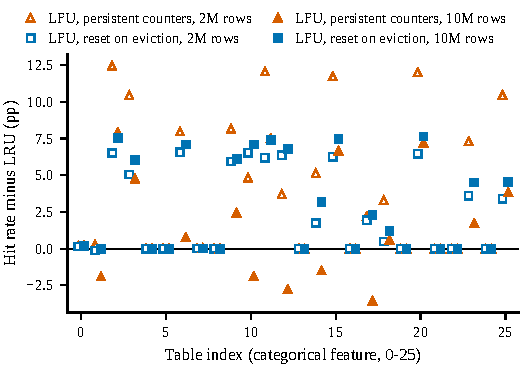
\includegraphics{fig_pertable}
\caption[]{Per-table caches of 256 vectors: hit rate of each LFU variant minus that of LRU, per table, at 2M (open)
and 10M rows (filled); zero means the same hit rate as LRU on that table. Source:
\src{results/P3/rows_*/figs/hit_rates.csv}, commit a84d9a9; script
\src{paper/v2/figs/fig_pertable.py}.}
\label{fig:pertable}
\end{figure}

Five tables (2, 3, 11, 15 and 20) have at least 150,000 distinct values at both trace lengths. Fig.~\ref{fig:large}
shows them combined: at 64 vectors per table, reset-on-eviction LFU, W-TinyLFU and ARC are well above LRU, and
Belady's bound stays above every online policy at every capacity shown.

\begin{figure}[t]
\centering
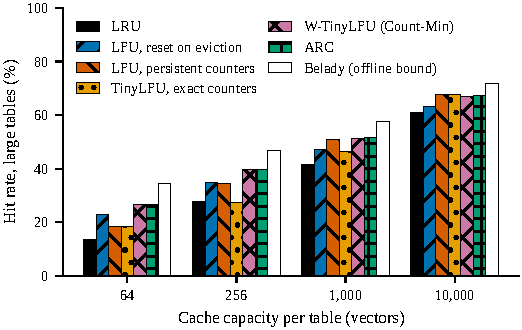
\includegraphics{fig_large}
\caption[]{Per-table caches, the five large tables (2, 3, 11, 15, 20) combined: hit rate by policy and capacity,
10M rows. Source: \src{results/P3/rows_10000000/figs/hit_rates.csv} and \src{zipf_per_table.csv} (commit a84d9a9);
script \src{paper/v2/figs/fig_large.py}.}
\label{fig:large}
\end{figure}

\textbf{Shared cache.} With one cache for all tables the picture changes (Fig.~\ref{fig:shared}). At 256 entries,
reset-on-eviction LFU beats LRU at both trace lengths (47.6719\% vs.\ 41.4010\% at 2M, 48.1592\% vs.\ 41.2640\% at
10M), and it does so at every capacity tested. The persistent-counter variant is below LRU at 256 entries at both
lengths (41.0006\% and 38.4896\%) and at 1,000 entries at 10M rows (52.9099\% vs.\ 53.4740\%); it is above LRU at
10,000 and 100,000 entries, and at 100,000 entries it has the highest hit rate of all policies (92.5839\% and
92.3924\%). At 256 and 1,000 entries, W-TinyLFU and ARC are the best policies. The persistent-counter variant also
loses the most from the shorter to the longer trace.

\begin{figure}[t]
\centering
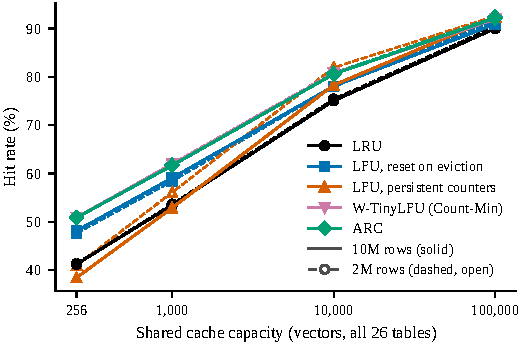
\includegraphics{fig_shared}
\caption[]{One cache shared by all 26 tables: total hit rate vs.\ capacity; 10M rows solid, 2M rows dashed with open
markers. Source: \src{results/P3b/rows_*/parts/*.csv} (commits c81407a, 79f9adc); script
\src{paper/v2/figs/fig_shared.py}.}
\label{fig:shared}
\end{figure}

\textbf{What the comparison shows.} The two LFU variants swap places between the two organisations: with per-table
caches the persistent-counter variant is ahead at 2M rows, with a shared cache it is behind LRU at small capacity
while the reset variant is ahead. In a shared cache, the tables compete for the same entries, and the persistent
variant keeps counts for every address it has seen; we did not isolate which of these causes the difference. ARC and
W-TinyLFU are the strongest online policies at small capacities in both organisations, but they need extra state
(ghost lists for ARC, a sketch and a window for W-TinyLFU); we did not measure that cost in hardware.

\section{Results: GPU Timing}\label{sec:res-gpu}
\textbf{Setup.} A synthetic model with 26 equal EmbeddingBag tables in PyTorch~\cite{paszke2019pytorch} (sum
pooling, one lookup per table and sample) followed by an MLP runs fp32 inference on one H100 and one H200 (script
\src{tools/profile_embedding.py}). Table rows are $10^{6}$ or $10^{7}$, the dimension 64 or 128, the batch 64 to 8192, with
uniform, Zipf and Criteo-hashed indices. Timing uses CUDA events only: the profiler \texttt{ncu} was not available
on the H100 node and refused to collect counters on the H200 node (\texttt{ERR\_NVGPUCTRPERM}), so there are no
hardware counters, and nothing here shows memory-boundedness or DRAM traffic. On the H100, 40 of 160 configurations
were skipped because the $10^{7}$-row, dimension-128 tables did not fit in GPU memory.

\begin{figure*}[t]
\centering
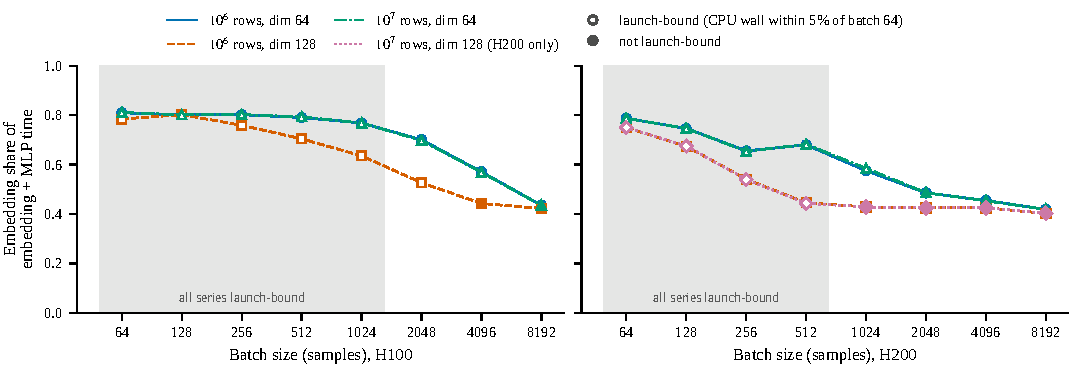
\includegraphics{fig_profile}
\caption[]{Median embedding share of embedding + MLP time vs.\ batch size, Criteo-hashed indices, fp32 inference on one
H100 (left) and one H200 (right); CUDA events only, no hardware counters. Open markers: launch-bound (CPU wall time per
iteration within 5\% of that at batch 64 for the same rows, dimension and index pattern). On the H100, 40 of 160
configurations were skipped for memory ($10^{7}$ rows, dimension 128). Source: \src{results/P4/h100_413621/results.csv},
\src{results/P4/h200_413622/results.csv} (commit daf1601); script \src{paper/v2/figs/fig_profile.py}.}
\label{fig:profile}
\end{figure*}

\textbf{Launch-bound region.} We call a configuration launch-bound if its CPU wall time per iteration is within 5\%
of the batch-64 value for the same tables and index pattern. Up to batch 1024 on the H100 and 512 on the H200 every
series in Fig.~\ref{fig:profile} is launch-bound: there the share is a share of kernel-launch time, not of lookup
cost. At batch 8192 the embedding share is 0.4224--0.4553 on the H100 and 0.4024--0.4358 on the H200 over all
configurations that ran. The model has 26 tables of equal size; production models have tables of very different
sizes, so these shares are not a statement about any production model.

\section{Results: Controller Hardware}\label{sec:res-hw}
\begin{figure*}[t]
\centering
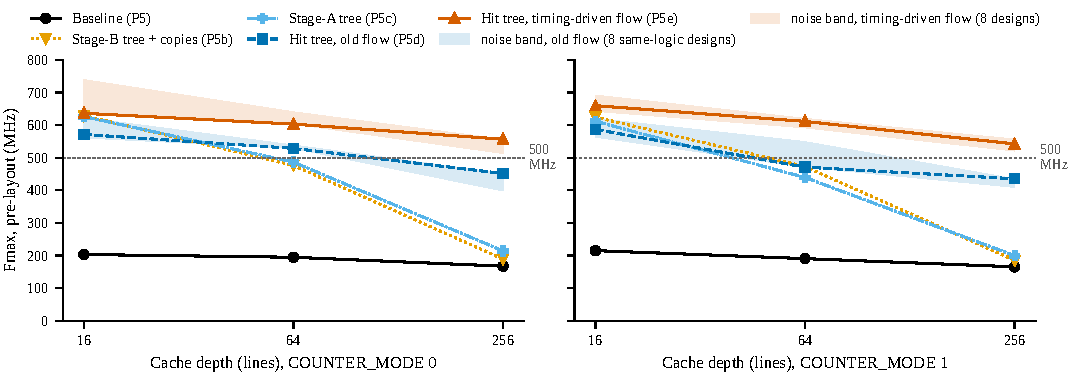
\includegraphics{fig_fmax}
\caption[]{Pre-layout Fmax on NanGate45 (not TSMC) of the 1\,GHz netlists vs.\ depth for each design iteration:
baseline, Stage-B reduction tree with address copies, Stage-A reduction tree, hit-index priority tree with the
earlier flow, and the same RTL with the timing-driven flow. Shaded: min--max Fmax of 8 designs with identical logic
(flow noise) for the two flows. Source: \src{results/P5*/d*_m*_1000MHz/sta.txt} and the noise-floor designs listed in
\src{results/P7/TABLES.md}; final RTL tag \src{rtl-v2-final}, flow commit 37c353c; script \src{paper/v2/figs/fig_fmax.py}.}
\label{fig:fmax}
\end{figure*}

\textbf{Design iterations.} Fig.~\ref{fig:fmax} follows the controller through three RTL changes and one flow change.
The baseline reached 203.1, 194.7 and 167.4\,MHz at depths 16, 64 and 256 (mode 0). Replacing serial minimum and
priority loops by balanced trees raised depth 256 to 451.2\,MHz with the earlier flow; the timing-driven flow then
gives 636.1, 603.0 and 556.6\,MHz on the same RTL. The noise bands are wide: with the earlier flow the 8 same-logic
designs spread by 1.96\% to 16.62\% in Fmax, with the current flow by 4.92\% to 16.23\%, so differences of that size
between two designs are not evidence of a design effect.

\begin{table}[t]
\centering
\caption[]{Final controller (tag \src{rtl-v2-final}) on NanGate45, timing-driven flow, pre-layout. Fmax from the
1\,GHz netlists; the 500\,MHz column is the netlist synthesized for 500\,MHz; noise = Fmax spread of 8 same-logic
designs. Area = sum of cell areas; no power analysis.}
\label{tab:synth}
\setlength{\tabcolsep}{2.5pt}
\begin{tabular}{rrrrrrlr}
\toprule
Depth & Mode & Cells & FFs & Area ($\mu$m$^2$) & Fmax & 500\,MHz & Noise \\
\midrule
16 & 0 & 11,466 & 2,957 & 26744.438 & 636.1 & met & 16.23\% \\
16 & 1 & 11,057 & 2,957 & 26626.866 & 659.5 & met & 7.71\% \\
64 & 0 & 37,939 & 10,431 & 94385.578 & 603.0 & met & 6.24\% \\
64 & 1 & 38,692 & 10,431 & 95100.852 & 611.2 & met & 4.92\% \\
256 & 0 & 149,620 & 40,225 & 369529.860 & 556.6 & $-$0.0357\,ns & 8.53\% \\
256 & 1 & 150,254 & 40,225 & 370226.514 & 542.3 & $-$0.0015\,ns & 7.02\% \\
\bottomrule
\end{tabular}\\[3pt]
\parbox{\columnwidth}{\footnotesize\raggedright Fmax in MHz; FFs = flip-flops. 500\,MHz: ``met'' or the worst negative slack of
the 500\,MHz netlist. At depth 256 the shortfall is far inside the noise, so meeting 500\,MHz is not demonstrated.
Source: \src{results/P7/TABLES.md} (P5e, noise floor), generated from \src{results/P5e/new/d*/sta.txt} and
\src{stat.txt} (commit 37c353c) and the noise-floor designs.}
\end{table}

\textbf{Final controller.} Table~\ref{tab:synth} lists the final design. The 500\,MHz netlists meet 500\,MHz at
depths 16 and 64 in both modes. At depth 256 they miss by 0.0357\,ns (mode 0, 491.2\,MHz) and 0.0015\,ns (mode 1,
499.6\,MHz); these shortfalls are far inside the noise of 8.53\% and 7.02\%, so whether depth 256 meets 500\,MHz is
not demonstrated either way. Compared
with the earlier flow on the same RTL, the timing-driven flow uses 1.52\% and 1.94\% more area at depth 64 and
2.81\% and 2.01\% more at depth 256, and at depth 64 it has more nets that violate the slew or capacitance limit
(2 to 7 in mode 0, 3 to 6 in mode 1; the reset net, which drives every flip-flop before any buffer tree is built, is
excluded from these counts). A layout flow would buffer such nets, and timing would change.

\begin{table}[t]
\centering
\caption[]{Verification of the final controller. GLS = functional gate-level simulation, zero delay, cell models
generated by Yosys from the liberty file.}
\label{tab:verif}
\setlength{\tabcolsep}{3pt}
\begin{tabular}{p{0.3\columnwidth}p{0.62\columnwidth}}
\toprule
Check & Result \\
\midrule
Mutation (RTL) & 113 mutant runs killed by the unit tests, 10 more by the lockstep check, 33 runs of equivalent mutants \\
GLS, unit tests & all 7 tests pass on the depth-16 and depth-64 netlists (Icarus 12) and on the depth-16 and
depth-256 netlists (Icarus 11) \\
GLS, lockstep & 12 netlists, 200,000 random cycles each: 0 mismatching cycles on all 5 outputs, no X \\
Equivalence & depth 16 only: 4 netlists, 2977 of 2977 equivalence points proven \\
\bottomrule
\end{tabular}\\[3pt]
\parbox{\columnwidth}{\footnotesize\raggedright Source: \src{results/P7/TABLES.md} (P5f, mutation), generated from
\src{results/P5f_gls/} (commits d7a2b54, 18b6aeb, 215d493) and \src{results/P5d/mutation.txt} (tag rtl-v2-final).}
\end{table}

\textbf{Verification.} Table~\ref{tab:verif} summarises the checks. In the lockstep run the netlist and the RTL see
the same random requests and fills; the hit flag, response valid, response data, fill request and fill address are
compared every cycle. The gate-level simulation has no delays, so it checks the logic of the netlists, not their
timing. The equivalence proof treats the asynchronous reset as synchronous and starts the induction from matched
registers being equal; it completed at depth 16 only.

\section{Limitations}
\begin{itemize}
\item \emph{Data}: only the first 2,000,000 and 10,000,000 rows of the 45,840,617-row file; results changed between
the two lengths (most for the persistent-counter LFU), so longer traces may change them again.
\item \emph{Organisation}: per-table and shared results are not comparable one to one, and the shared order of
accesses within a row is a modelling choice.
\item \emph{Simulator vs.\ RTL}: tie-break and counter width differ (Section~\ref{sec:rtl}); the RTL was not replayed
on the traces; there is no RTL for persistent per-address counters, ARC or W-TinyLFU.
\item \emph{GPU timing}: CUDA events only, no hardware counters; a synthetic model with 26 equal tables and one
lookup per table; one GPU of each type; small batches are launch-bound.
\item \emph{Hardware}: NanGate45, not TSMC; pre-layout with a wire-load model and ideal clock; area is a sum of cell
areas; no power; Fmax differences below the noise floor are not meaningful; the timing-driven flow was tuned on a
single depth-16 pilot without ablation, uses up to 2.81\% more area, and adds slew/capacitance violations at depth 64.
\item \emph{Verification}: gate-level simulation is zero-delay; equivalence is proven only at depth 16.
\item \emph{Earlier work}: an earlier gem5 study of this project (a CPU with DDR4, not a GPU~\cite{binkert2011gem5})
is not reproduced here; the statistics of most of its runs are not available, and we use none of its numbers.
\end{itemize}

\section{Conclusion}
On Criteo traces, frequency information helps embedding caches, but how it is kept matters, and the answer depends
on whether tables share a cache. Per-table caches favour both LFU variants over LRU; a shared cache favours LFU that
resets counts on eviction and penalises the variant that keeps them, at small capacities. ARC and W-TinyLFU are the
strongest online policies at small capacities, at a hardware cost we have not measured. The synthesizable controller,
whose default mode belongs to the reset-on-eviction family, reaches 542.3--659.5\,MHz pre-layout on NanGate45 and
matches its RTL at gate level. Next steps are replaying the traces through the RTL, longer traces, and a hardware
estimate for ARC and W-TinyLFU.

\bibliographystyle{IEEEtran}
\bibliography{refs}

\end{document}
